%% ACM Computing Surveys format for this manuscript.
%% Based on ACM's official acmsmall template and the organization of
%% "Explainable AI (XAI): Core Ideas, Techniques, and Solutions."
%%
%% Compile this file from either the project root or the figures directory.
%% For a submission-only single-column review copy, ACM currently recommends
%% replacing the class options below with: \documentclass[manuscript,review]{acmart}

\documentclass[acmsmall,screen,review]{acmart}

% Page layout and typography
% \usepackage[margin=1in]{geometry}
% \usepackage[T1]{fontenc}
\usepackage{lmodern}
\usepackage{microtype}

% Scientific writing
\usepackage{amsmath,amssymb}
\usepackage{graphicx}
\usepackage{booktabs}
\usepackage{tabularx}
% \usepackage{cite}

% Links and references
% \usepackage[hidelinks]{hyperref}

\AtBeginDocument{%
  \providecommand\BibTeX{{Bib\TeX}}%
}

%% Journal metadata known at manuscript preparation time.
%% ACM supplies volume, issue, article number, DOI, dates, and rights metadata
%% after acceptance; do not invent those values for a submission draft.
\acmJournal{CSUR}
\setcopyright{none}
\settopmatter{printacmref=false}
\citestyle{acmnumeric}

\title[Single-LLM Versus Multi-Agent Debate Systems]
  {Single-LLM Versus Multi-Agent Debate Systems for Scientific Hypothesis Generation}

\author{Soumik Bhattacharyya}
\email{mde2026005@iiita.ac.in}
\affiliation{%
  \department{Department of Information Technology}
  \institution{Indian Institute of Information Technology Allahabad}
  \city{Prayagraj}
  \state{Uttar Pradesh}
  \country{India}
}

\begin{document}

\begin{abstract}
Large language models (LLMs) have been used for generating scientific hypotheses, literature search and integration, evaluation of possible explanations, and experiment design. The two main approaches of LLM usage are either single-LLM based systems using one model via prompts, retrieval, self-reflection, or tool use, or multi-agent systems using multiple instances of the model interacting via debate, specialization of roles, iterative review, or convergence. In this review we study comparison of these two paradigms of scientific hypothesis generation. Instead of assuming that multi-agent interactions are inherently better, the literature is analyzed through the lens of five themes: hypothesis generation and novelty, evidence grounding and verification, criticism and debate, quality evaluation of science, and autonomous research workflow integration. We find that from our reviewed studies single-LLM systems are simpler, cheaper, more controllable and perform well if provided with right literature or domain-specific tools. Multi-agent systems are good to explore, criticize, and compare the alternate ideas especially if agents are diverse and with complimentary roles. The downsides of the debate for costs and problems of sharing model errors, sycophancy, early convergence and problem drift can be significant. Thus, a promising approach is to use a conditional hybrid solution consisting of independent generation, followed by evidence retrieval, targeted adversarial review, selective debate, and experimental validation. Major gaps exist in the area of standardized benchmarks, attribution of multi-agent gains via causality, calibration, measure of diversity, and real world lab validation.

\end{abstract}

\keywords{large language models, scientific hypothesis generation, multi-agent systems, debate, literature-based discovery, autonomous science, evaluation}

\maketitle

\section{Introduction}
\label{sec:introduction}

In order to make scientific discoveries, one needs to be able to link observations, find regularities, formulate explanatory hypotheses, and decide which hypotheses would be worth the effort to test empirically. The use of computational methods to make discoveries has been around for quite a while. Initial systems including BACON, a computational scientific-discovery system that discovers regularities in observations and generates candidate scientific laws, showed that programs can search observations for regularities and represent them in the form of candidate scientific laws; literature-based discovery showed that useful knowledge can be discovered by linking distributed information across otherwise independent bodies of research \cite{swanson1986undiscovered,langley1987scientific}.

Recently, this problem has been scaled up and made flexible by the introduction of recent LLM platforms. An LLM might be able to summarise literature, suggest mechanisms, merge concepts, design experiments and tweak ideas in natural language, rather than relying solely on manually written discovery rules. There have been studies that focus on direct hypothesis generation \cite{zhou2024hypothesis,yang2024large} and studies that concentrate on the entire research automation process including literature retrieval, coding, experimentation, and manuscript preparation \cite{lu2024ai,yamada2026towards}. Single-LLM can also serve as a relatively simple and lower-cost solution for scientific reasoning assistance, as it can be used as a simple tool that can generate and refine scientific ideas without the need for coordination between multiple agents.

Simultaneously, scientists have started introducing more than one model, one model interacting with another. Here one agent might create ideas, another might be a critic, another might evaluate novelty, another might evaluate feasibility, another might evaluate evidence, and another might evaluate experimental design. Multi-agent debate is appealing because science is not just a process of making explanations, it's also a process of challenging explanations. Several agents can offer a variety of views, and offer multiple chances to critique and revise. This interaction on the other hand is expensive in terms of computation and engineering and can also lead to agreement with no correctness, especially if agents have similar biases or tend to confirm non-supported assertions.

The trade-offs highlight that it does not have to be a trade-off between a single LLM versus a full-scale multi-agent system. The low costs and ease of single-LLM methods and the variety and critical analysis provided by multi-agent systems could be synergized or optimized. A hybrid model may then be implemented to the proper degree of interaction according to the scientific task, research question or stage of the hypothesis formation. The real question is then not only which are multiple agents better than a single agent, but when is it best to use a combination of single-LLM and multi-agent capabilities for scientific hypothesis generation.

The question is explored in this review under the following research question: \textbf{What are the differences in the capacity to generate new, valid, feasible and experimentally useful scientific hypotheses between models of single-LLM and multi-agent debate; and what design choices lead to different advantages?} The review examines systems that generate scientific ideas or hypotheses, while also considering related work on reasoning, scientific agents, and automated experimentation.


\subsection{Scientific hypothesis generation with LLMs}
\label{subsec:scientific-hypothesis-generation}
A scientific hypothesis is a formal, testable statement or prediction about a relationship among observations, variables, mechanisms or interventions. For practical research, a useful hypothesis should meet a number of requirements: it should be novel, it should relate to existing evidence, it should be scientifically plausible, operationally testable, and it should have a possible impact. These criteria may be in opposition. A very novel idea may be poorly grounded; a very well established idea from existing literature may be incremental.

Traditionally, the computational discovery systems have been able to detect candidate regularities and then evaluate the candidate regularities. BACON-like systems were used to find patterns in the data and to create laws \cite{langley1987scientific}. In contrast, literature based discovery approaches identified meaningful connections in the text or bibliographic space \cite{swanson1986undiscovered}. Unlike well-established rule-based discovery, LLM-based systems integrate components of these functions by providing a flexible language interface for these functions.

An LLM works by approximating a probability distribution over the next possible tokens, given the rest of the context. The simplified form of the probability of a sequence generated is
\begin{equation}
P\left(y_{1:T}\mid x\right)
=
\prod_{t=1}^{T}P\left(y_t\mid y_{<t},x\right).
\end{equation}
where $x$ is the input context, $y_t$ is the token generated at position $t$ and $y_{<t}$ is all the tokens generated before $t$. Therefore, the model need not explicitly learn a science law or make a formally correct inference in order to be able to generate a hypothesis. Rather, the model can make new guesses about what is happening by recombining patterns and relationships stored in its learned parameters and provided in the context.

The question I want to pose here is, is probabilistic text generation a scientifically valid foundation for hypothesis generation? The answer will depend on the definition of ``sound. Prospecting for probabilities does not prove a hypothesis scientifically true, causally valid or even true at all. A high probability continuation could simply be a trend that is common in the training set. LLMs can then generate plausible yet unprovable hypotheses in language. This restriction is especially significant because the probability assigned to a sequence that is generated is not a probability that the scientific statement itself is true.

Scientific hypothesis generation is an exploratory process, however. A hypothesis is a suggestion that is to be tested, not a statement that is believed to be true. In the recent literature, it has been proposed that the probabilistic and sometimes counterintuitive outputs of LLMs could be beneficial for proposing candidate hypotheses, which are then tested with scientific evidence or experiments.In recent work it has been suggested that the outputs of LLMs, when probabilistic, or sometimes unexpected, could be helpful for proposing candidate hypotheses, which are subsequently tested with scientific evidence or experiments. Zhou et al. show that LLM-generated hypotheses can be further refined with observed data, and that they can boost predictive ability over few shot prompting in various benchmark scenarios \cite{zhou2024hypothesis}. Laboratory validation also has advantages in providing supporting evidence for the feasibility of this approach: GPT-4 generated candidate drug combinations, some of which were subsequently shown to have positive experimental synergy, but the study noted some limitations in the quality of the explanations given with the drug combinations generated \cite{abdelrehim2025scientific}.

The scientific merit of an LLM-generated hypothesis should not be evaluated based on the likelihood of its generation alone. The LLM is an exploration of a rich space of candidate ideas; novelty, evidential grounding, plausibility, feasibility and experimental validity are evaluated independently of the LLM. The difference between single-LLM systems and multi-agent systems is a key consideration: the primary issue isn't which system can write the most believable text, but which system can reliably transform the text it writes into a scientifically useful hypothesis.

\subsection{Single-LLM systems}
\label{subsec:single-llm}

Single-LLM: One instance of the model acts as the primary generator and reasoner. It can be improved by prompt engineering, chain of thought reasoning, retrieval-augmented generation, external means, memory, self-critique, or iterative refinement. Self-Refine and Reflexion show the bigger picture: that a model can produce an output and then use feedback or memory to refine that output \cite{madaan2023selfrefine,shinn2023reflexion}.

The single-LLM paradigm ought not to be confused with a single prompt. They can be internal or sequential multiple stages in a single model. The unique aspect is that the stages are not managed by individually instantiated agents with different roles or instructions, but by one model.


\subsection{Multi-agent debate systems}
\label{subsec:multi-agent}

Multi-agent systems partition the process into multiple instances of models or agent roles. The usual process is to have proposals made and critiqued by someone other than the proposer, to have a response or rebuttal, to have proposals synthesized, and to be ranked. Debate can be open-ended, role based, or facilitated by a facilitator. The aim is to broaden the search and bring about explicit disagreement before making a final decision.

The study of multi-agent debate focused on factuality and reasoning, not exclusively on the scientific ideation. It has been reported by Du et al. that debate can be a helpful strategy to improve performance on some reasoning and factuality tasks \cite{du2024improving}. Later, however, it was found that multi-agent debate is not consistently better than simpler baselines and is configuration-, cost-, and task-sensitive \cite{smit2024mad}. This adds to a body of research directly applicable to the scientific hypothesis generation where the quality of the evaluation process may be more important than the number of agents.



\section{Thematic Literature Review}
\label{sec:thematic-literature-review}

\subsection{Theme 1: Generation, novelty, and exploration}
\label{subsec:generation-novelty-exploration}

A prominent role that LLM can play is to distill from vast scientific text candidate research directions. Zhou et al. investigate hypothesis generation using LLMs, and demonstrate the ability to use prompts and data-driven formulations to generate candidate hypotheses \cite{zhou2024hypothesis}. Similarly, Yang et al. study automated discovery of scientific hypotheses in the open domain, showing that LLMs can produce results beyond simple question answering to research-oriented generation \cite{yang2024large}.

Novelty is hard to define and measure, but. A statement that has been generated can be linguistically atypical but trivial, known, or untestable. To cure this, SciMON (Scientific Inspiration Machines for Optimizing Novelty) retrieves inspirations from scientific literature and optimizes candidate scientific ideas for novelty \cite{wang2024scimon}. The design suggests that novelty should be considered as a search goal that is based on literature, rather than as a feature that only comes from the text of the output.

This distinction is confirmed by human evaluation studies. Si et al. test the LLM-generated research ideas with a large community of NLP researchers and discuss the dimensions of novelty and feasibility \cite{si2025novel}. The work indicates that LLM-generated ideas can be competitive in some ways, but it also highlights the need for expert judgment, including implicit disciplinary knowledge, in determining research quality, which encompasses the assessment of the practical feasibility of the research to potentially benefit the field.

The multi-agent systems can potentially enhance exploration by having multiple agents suggest alternatives prior to synthesis. Under their evaluation protocol \cite{su2025many}, a multi-agent scientific-ideation system can enhance the quality of the ideas compared to single-agent baselines, according to Su et al. The probable mechanism is not just in parallel text generation. Multiple agents may traverse multiple conceptual paths and expose assumptions, and may also retain alternatives that one generation may be too hasty in discarding.

However, simply more agents does not necessarily mean more useful diversity. When all agents have the same model and prompts and the same retrieval corpus and priors, the proposed answers might be quite similar. Therefore, diversity needs to be planned for in independent sampling, role variation, different evidence views, and/or explicit disagreement objectives.


\subsection{Theme 2: Evidence grounding, literature retrieval, and verification}
\label{subsec:evidence-grounding}

The fluency of scientific hypotheses is not enough to assess them. These have to relate to observations/observation data, previous research, mechanism and practical measurement. Grounding in literature is therefore pivotal in both single-agent and multi-agent systems. Zhou et al. highlight the need for scientific data and context to be used in hypothesis generation \cite{zhou2024hypothesis} and SciMON explicitly searches the literature for ideas to support novelty \cite{wang2024scimon}.

Adding evidence grounding can enhance the factuality and minimise the possibility for an LLM to come up with unsupported mechanisms. It also makes the hypothesis created by the system more useful to the researchers, as it can point out evidence that supports the hypothesis, contradicts it, and identifies experiments the researchers will need to conduct to confirm the hypothesis. But, just because you can retrieve something doesn't automatically mean it's correct. A model can misunderstand a paper, quote evidence without it directly supporting the claim, or add evidence from conflicting settings.

In fact, the distinction between single-LLM and multi-agent approaches may not be that of what the model can and cannot do. A single LLM can be broken down into a series of steps: retrieval of evidence, hypothesis generation, proposal evaluation, and proposal revision. These roles are made explicit in multi-agent architectures, where they are attributed to different interacting agents. Such separation can bring with it special prompts, independent criticism, different contexts, or parallel reasoning paths, but also add more computational and coordination costs. Whether there is a benefit in the use of multi-agent systems will thus depend on the performance of the evaluation process when the additional diversity and specialization are combined with sequential use of one model.

The AI co-scientist profession serves as an example of a more general generate--debate--evolve pattern, in which candidates' ideas are continually evaluated and improved over time \cite{gottweis2025towards}. The Virtual Lab also highlights the importance of aligning the tasks of agentic reasoning with experimental validation, instead of just considering textual matching as the ultimate goal \cite{virtuallab2024}. The above approaches are not intended as a rule to be followed, they simply represent examples of how structured interaction and iterative evaluation can be combined in scientific discovery.

The same basic limitations on evidence can also be passed on through both approaches. Single-LLM pipelines, or all downstream agents, may reason over the same missing evidence if the initial retrieval fails. Similarly, other agents can be incorrect and reproduce these without basis. A good architecture should then track provenance, differentiate retrieved evidence from model inferences and demand that uncertainty is explicitly stated.


\subsection{Theme 3: Critique, self-reflection, and debate}
\label{subsec:critique-debate}
The best theoretical justification for multi-agent debate is the critique. There is a need to recognize hidden assumptions, alternative explanations, confounding variables and weaknesses in experimental design in scientific reasoning. Self-critique can be done through iterative prompting with Single-LLM systems. Self-Refine is based on the model of revision \cite{madaan2023selfrefine} driven by feedback, while Reflexion incorporates verbal feedback and memory to aid future attempts \cite{shinn2023reflexion}. These can be effective if the model has the ability to identify its mistakes.

But self-critique is not a different type of criticism. The same model that made the hypothesis provides the interpretation, criteria and final judgment. May rationalize without challenging the first answer. Multi-agent debate solves this issue by splitting the proposals and criticisms among agents. In general, they demonstrate that debate is beneficial for some aspects of reasoning and factuality \cite{du2024improving}.

The complexity and complexity of scientific ideation add to this. Even in cases where everyone agrees to the facts, debate participants can differ on questions of novelty, feasibility and importance. Multi-agent debate is not always more effective than self-consistency or ensembling, and performance may be influenced by the debate strategy and task, warns Smit et al. \cite{smit2024mad}. This is particularly true of scientific hypotheses, where the answer is sometimes not readily known.

Debate can also lead to social dynamics that are not desirable among agents. Early proposals may be converged to because of their frequent repetition, perceived as authoritative, or delivered with high confidence. Consensus can hence, be a poor indicator for the scientific validity. It's probably best to have an adversarial, but structured, debate by requiring agents to provide evidence, set out conditions that could be used to prove that evidence is incorrect, suggest alternatives, and keep the disagreement unresolved.

\subsection{Theme 4: Evaluation of scientific quality}
\label{subsec:evaluation-quality}

The main obstacle in the literature is evaluation. Common dimensions include novelty, relevance, significance, feasibility, validity, clarity and potential impact. These dimensions go hand in hand but not interchangeable. A hypothesis may be new, but improbable; possible, but uninteresting; or interesting but previously accepted.

IdeaBench suggests a research-idea generation approach based on benchmark and points out the need for systematic assessment of research ideas \cite{guo2025ideabench}. The biomedical evaluation of Qi et al. also covers multiple aspects such as novelty, relevance and significance and verifiability \cite{qi2024biomedical}. This kind of work is crucial because it takes the evaluation out of the hands of an LLM-judge.

A higher level of evidence is experimental validation. Boiko et al. demonstrate autonomous chemical research with LLMs, where they show the use of language-based reasoning that can be linked to laboratory procedures \cite{boiko2023autonomous}. The breast-cancer lab study is another such case study of experimental testing of such combination-drug hypotheses, generated by LLM's, in a lab setting \cite{scientific2025laboratory}. These studies do not demonstrate that an architecture is always superior, but they do suggest that the usefulness of a scientific idea comes down to whether or not it survives the experiments.

Multi-agent systems can enhance the evaluation process by using individual agents for novelty, feasibility, evidence, and risk. But this is a decomposition that can lead to false precision. There may be several agents with scores that appear strict but have the same model biases. The evaluation should, therefore, incorporate external evidence, expert judgment, prospective prediction, and, if possible, experimental success. As hypothesis generation is integrated into the overall autonomous research workflows, these evaluation challenges become more relevant.


\subsection{Theme 5: From hypothesis generation to autonomous science}
\label{subsec:autonomous-science}

More and more, the process of hypothesis generation is being considered as part of a complete research cycle.
The AI Scientist aims to take over idea generation, coding, experiments, analysis and paper.
writing \cite{lu2024ai}. The AI co-scientist and the systems that relate to it carry on this concept across several layers.
For the first time, agents, iterative debate and evidence-based evolution \cite{gottweis2025towards} are combined.

These systems imply that the single/multi binary is becoming less meaningful in practice. A
single agent can call tools and perform multiple internal roles, a multi-agent system can use
an effective coordinator, who acts like a single decision maker. The closer the more useful comparison is
therefore functional: how many independent searches occur, how criticism is generated, how
Evidence is validated and how final decisions are made.

There are also weaknesses in end-to-end automation. Generate autonomous systems
Improperly develop ideas, conduct experiments improperly, or write manuscripts that look
While the paper's methodology is flawed, it remains coherent.Although the methodology is weak, the paper can still be considered coherent \cite{lu2024ai,yamada2026towards}. This reinforces
The need for human monitoring of and explicit validation gates.


\section{Comparison of Existing Approaches}
\label{sec:comparison}

A variety of metrics should be taken into account when evaluating the performance of a single-LLM and multi-agent systems, rather than relying on just one score. The relevant differences between the systems available in the literature are summarized and discussed in detail below in Table~\ref{tab:system-comparison} and are summarized below.The following are some of the key differences between the systems available in the literature, summarized in Table~\ref{tab:system-comparison} and discussed below.

\begin{table}[htbp]
  \centering
  \caption{Comparison of single-LLM and multi-agent systems for scientific hypothesis generation.}
  \label{tab:system-comparison}
  \small
  \renewcommand{\arraystretch}{1.2}
  \begin{tabularx}{\textwidth}{@{}>{\raggedright\arraybackslash}p{0.18\textwidth}
                                  >{\raggedright\arraybackslash}X
                                  >{\raggedright\arraybackslash}X@{}}
    \toprule
    \textbf{Dimension} & \textbf{Single-LLM Systems} & \textbf{Multi-Agent Systems} \\
    \midrule
    Cost and efficiency & Lower computational and orchestration cost
                        & Higher token use, latency, and coordination cost \\
    Search breadth      & Multiple samples possible through prompting
                        & Explicit parallel exploration of diverse ideas \\
    Criticism           & Self-reflection and internal critique
                        & Independent, role-based criticism and debate \\
    Evidence use        & Single evidence path; simpler pipeline
                        & Evidence work can be distributed across agents \\
    Reproducibility     & Easier to reproduce
                        & Depends on agent roles, topology, and debate configuration \\
    Scalability         & Scales through model and tool improvements
                        & Scales through additional agents, with coordination costs \\
    Validation          & Requires external experimental validation
                        & Also requires external experimental validation \\
    \bottomrule
  \end{tabularx}
\end{table}


\begin{itemize}
  \item \textbf{Cost and efficiency.} Single-LLM systems generally require fewer calls to the model, and are more easily deployable. Expanding the number of agents leads to more tokens, latency, orchestration complexity and often the number of retrieval operations.

  \item \textbf{Search breadth.} While it is possible for one model to generate several samples, multi-agent systems explicitly train parallel exploration. They're focused on if the agents actually are diverse.

  \item \textbf{Criticism.} It's a simple and inexpensive method of self-critique, but multi-agent criticism might be more difficult. Provide own opinions more freely. Neither guarantees correctness.

  \item \textbf{Evidence use.} There are benefits to using both paradigms in terms of retrieval, and tools. Evidence work can be broken up into a number of tasks, and there are common failures of evidence retrieval that can be shared among agents.

  \item \textbf{Reproducibility.} Single-LLM pipelines have the advantage of being more easily defined and reproduced. The roles of agents as well as the communication topology, stopping rules, and the order in which the agents debate are important influences on multi-agent results.

  \item \textbf{Scalability.} Single-LLM systems scale by making the model larger, more specialized prompts, and making use of tools. Do not get into the trap of scale out by increasing agents, coordination costs and convergence problems.

  \item \textbf{Validation.} These architectures are not complete without validation: It's better to have a text consensus than laboratory or prospective validation.

\end{itemize}

Overall, the literature indicates that there is no consensus that MultiAgent debate is better.
Multi-agent systems appear to be most useful if the task can be approached via independent search, specialization, or via multiagent communication.
Comparing and criticizing other possible explanations. Single-LLM systems continue to be appealing.
Where cost, speed, repeatability and good tool integration is more important.They become apparent when the systems are considered as having distinct functions, rather than distinct architectures.



\subsection{A functional comparison of system components}
\label{subsec:functional-comparison}
Both of the paradigms can contain generation, retrieval, critique, ranking, memory and tool use. The difference is in the allocation of these functions. A single-LLM pipeline typically involves a single model that is used to perform multiple tasks in a series or via structured prompts. The functions will be split in a multi-agent pipeline where the agents will communicate with each other using messages or shared artifact. The number of agents therefore, is not a good indicator of sophistication in the architecture. Figure~\ref{fig:functional-allocation} illustrates this functional allocation, either in a single-LLM pipeline or a multi-agent pipeline.

\begin{figure*}[t]
  \centering
  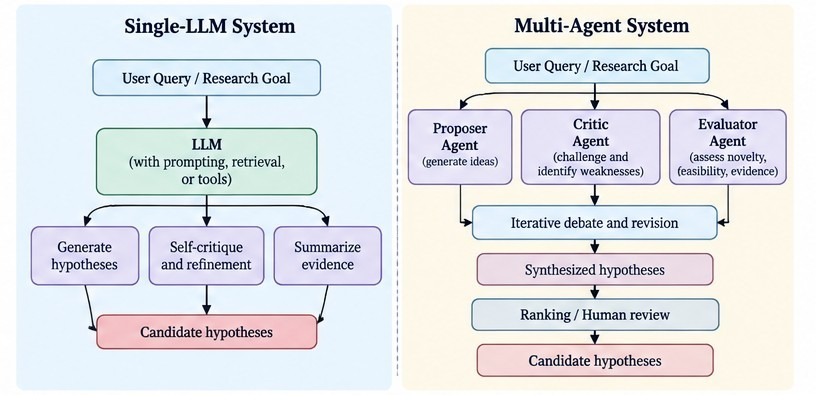
\includegraphics[width=\textwidth]{figures/functional-comparison.jpg}
  \caption{Scientific Hypothesis Generation with Single-LLM vs Multi-Agent Systems. Single-LLM systems use a single model, with prompting, retrieval or tool usage, and multi-agent systems use specialised agents to debate, critique and iteratively revise candidate hypotheses.}
  \label{fig:functional-allocation}
\end{figure*}

Candidate generation is the first working element. Multiple candidates can be generated from a single model, by using temperature sampling or prompt variation or by repeating calls. This can be a decent approximation of the number of agents, however the prospects are often produced utilizing comparable presumptions in regards to the population. Making independence explicit is one way to have multiple agents with different starting points, disciplinary perspectives or subsets of evidence. This benefit is greatest when the agents are not deterred from first presenting alternative explanations.

Evaluation is the second part. One LLM system can ask the model to perform novelty, plausibility and feasibility scoring but the scores can be correlated with generation internally with the original generation. In a multi-agent system, various aspects can be critiqued by different critics. One critic can examine to see if the claim is substantiated by the literature, another can see whether the proposed mechanism is sufficient or not, and another can develop a test to see if the claim is true. The downside of this decomposition is that it complicates the problem for a final controller that is supposed to resolve disagreements, since it is the problem of aggregation. The problem is how a final controller is supposed to resolve disagreements without obtaining some average of all the disagreements.

The third phase is in evidence management. In both paradigms, retrieval-augmented generation, citation tracing, structured notes, and tool calls are possible. Single-LLM systems generally have a shorter evidence chain, making it easier to audit them. Distributing retrieval and verification is possible with a multi-agent system, but the problem is to maintain the provenance information for each agent. The system can produce a polished synthesis that is difficult to analyze for evidence if the statement and the supporting paper do not already have a shared record of the evidence that exists in each paper.



\subsection{Where more agents can help---and why they may not}
\label{subsec:agents-benefits-limitations}

Part of the argument for having multiple agents is that the chance of common sense failures is reduced. When agents approach a problem separately, disagreement can uncover an assumption, or even a different mechanism. This is especially useful when dealing with open-ended science questions where there is seldom a clear cut answer that can be immediately determined. Nonetheless, multiple model instances are not guaranteed to result in independence if the design is one of the models.But note that multiple instances of the design is not guaranteed to produce independence if the design is one of the models. It is possible for agents to make the same error multiple times, if they use the same model, prompt template, retrieved papers, and evaluation rubric. However, there are also recent studies on multi-agent debate that demonstrate agents can reinforce each other and reach false consensus conclusions instead of correcting them \cite{choi2025debatevote}.

There's also the difference between constructive and disruptive debate. Productive disagreement is specific: an agent finds a missing control, asks a question about an interpretation of the cause, offers a test to differentiate two causal interpretations. Disagreements are pointless unless they're loud enough to be heard and support or refute points, rather than just restate them. Past research on multi-agent research dialogues indicates that agent diversity and interaction depth can influence the quality and diversity of the ideas generated, but not all aspects of the outcomes are necessarily enhanced by increased agent diversity and interaction depth \cite{ueda2025design}. A useful debate protocol should thus specify, for each of the critiques, the claim being attacked, the evidence or assumption under attack, and the implications for an experiment. This makes the discussion more traceable and minimises the possibility that the talkativeness will be confused as being of high quality in the sense of reasoning.

Yet another drawback is early convergence. Later agents may assume the hypothesis presented by one or more agents is correct and change it in superficial ways. This convergence can be efficient if the prevailing hypothesis turns out to be the right one, and it is risky if the initial one is not. Consensus and sycophantic agreement in multi-agent debate does not necessarily imply independent validation, as more agents does not necessarily mean more validation \cite{choi2025debatevote}. Therefore, scientific systems should maintain a few serious options until evidence based ranking and/or experimental testing shows why they should be eliminated.


\subsection{The role of human researchers in the comparison}
\label{subsec:human-researchers}

The competition between the single agent and the multi agent is not a replacement game between models and scientists. Human researchers bring in domain expertise, implicit standards of evidence, knowledge of practicalities and sense of what is important. It is not easy to fully quantify these contributions in automated scores. A single-LLM workflow allows the researcher to control the prompt, choose the sources, and review the resulting hypothesis. A multi-agent workflow also allows the researcher the ability to create roles, establish debate rules, settle disputes and approve experiments.

There is a particular importance of humans at the transition from the textual plausibility to the scientific action. A hypothesis might be interesting, but impractical because of unavailable equipment, an experiment that would be unethical, a confounder that is not being measured, or a sample size that is too large to allow the proposed test to be implemented. Breadth and structured criticism can be provided by an LLM in a human-in-the-loop design, yet with human control over interpretation, safety and experimental prioritisation. The system that works best for this is also the desired realistic evaluation target: that is, the value of a system may be evaluated not only by its stand-alone text but also by how much better a scientist's decision making is made.


\section{Research Trends and Developments}
\label{sec:research-trends}

\begin{enumerate}
  \item \textbf{Literature-grounded generation.} Systems are increasingly able to find papers, pick out evidence,
  Create constraints on generation and use scientific information
  \cite{zhou2024hypothesis,wang2024scimon,qi2024biomedical}.

  \item \textbf{Agent Specialisation.} Multi-agent systems specify roles like literature analyst, experimental designer and risk assessor. generator, critic, etc. to its agents.
  \cite{su2025many,gottweis2025towards}.

  \item \textbf{Closed-loop discovery.} Research systems are now increasingly linking hypothesis generation with coding, experimentation, analysis, and revision, which is referred to as closed-loop discovery.
  \cite{lu2024ai,yamada2026towards,gottweis2025towards,boiko2023autonomous}.

  \item \textbf{Benchmarking and structured evaluation.} Recent work emphasizes novelty, feasibility, validity, verifiability and impact, not fluency.
  \cite{si2025novel,guo2025ideabench,qi2024biomedical}.

  \item \textbf{Experimental validation.} Laboratory research is now underway to determine if LLM-generated ideas that have scientific value can be measured.
  \cite{virtuallab2024,boiko2023autonomous,scientific2025laboratory}.

  \item \textbf{Risk-aware scientific agents.} Safety and citation are increasingly becoming the concerns of scientific agents with a heightened sense of risk.
  The concepts of faithfulness, uncertainty, and human oversight are at the very heart of design.
  \cite{goo2026citation,safescientist2025,hong2024metagpt}.
\end{enumerate}


\subsection{A proposed evaluation framework}
\label{subsec:evaluation-framework}

The entire process of hypothesis generation should be rigorously evaluated. The first is novelty, against a time-stamped literature corpus with the help of experts' judgment. The second is scientific validity, whether the hypothesis is in accord with known observations, whether the causal/mechanistic explanation of the hypothesis is coherent. The third is feasibility, that is the existence of data, instruments, samples and realistic experiments. The fourth is predictive value: A good hypothesis should make a clear prediction that would be testable at a later time.

We have diversity as the fifth dimension. It is important to assess systems not only by what concept they generate but also by the variety of mechanisms and experimental directions they go through. Ten paraphrases don't equal ten discoveries. The sixth dimension is calibration that is, confidence should be proportional to the strength of the evidence. The seventh is efficiency such as token use, number of model calls, latency, retrieval cost and human review time. If these dimensions were reported in combination, then a system wouldn't seem better just because it required significantly more computing.

This is a useful experimental design: one or more LLM organizations with one generation, one or more LLM organizations with multiple candidates sampled, a multi-agent without debate, a multi-agent with structured debate. The same model family, literature access, evaluation instructions and budget for tokens (where applicable) should be applied to all conditions. The design would help distinguish whether any improvement observed is a result of the agents interacting or just because of the creation of more candidates.

Retrospective and prospective settings should also be distinguished when evaluating. In the case of retrospective evaluation, the system is presented with a set of documents from the literature, and its results are compared with the literature itself. This can be helpful for grounding and rediscovering, but can lead to the enticement of ideas that are already in the data. In prospective evaluation, ideas are formulated ahead of time and are evaluated against the results of future experiments and publications. Prospective evaluation is more complex, but is better at assessing the contribution of a system to real discovery.


\section{Challenges and Limitations}
\label{sec:challenges}

It is challenging to operationalise the concept of scientific novelty. Expert ratings can be subjective, expensive, and might reward unusual wording, while similarity-based measures can reward unusual wording. The existing literature is sometimes not sufficient to establish the scientific validity and it is necessary to carry out experiments or to predict the future. LLMs can also hallucinate mechanisms, references or experimental results. The risks are particularly high if a multi-agent system reiterates and reinforces an unbacked statement.

There are significant engineering costs associated with multi-agent debate. It performs well based on a number of agents, role prompts, communication structure, debate rounds, and aggregation method \cite{smit2024mad}. Minority ideas can be driven out of the system and agents can merge at an early stage on a likely but wrong explanation. Further, many evaluations are based on the use of LLM judges, which may be prone to common biases and exaggerate the strength of the systems.

Last, there is a lack of uniformity in the evidence: domains, prompts, models, datasets, expert panels and evaluation scales vary from study to study. The results obtained from biomedical hypothesis generation cannot be automatically transferred to the fields of chemistry, materials science, social or theoretical research. The comparison between single- and multi-agent systems is also confounded with different retrieval access, capability of models, and/or budgets of tokens.


\subsection{Reproducibility and reporting requirements}
\label{subsec:reproducibility}

In the future, it is important to report enough information about their implementation so that meaningful comparisons can be made. The required information for these details is the exact model and version, prompts, temperature settings, sampling settings, retrieval corpus and cutoff date, number of agents, descriptions of agents, communication topology, number of debate rounds, stopping criteria, judge prompts and total token expenditure. In the absence of such information, a perceived good thing could be a bad thing because of other differences in compute and/or information access.

Negative results and failure cases (such as rejections of hypotheses, unsupported citations, wrong interpretation of papers, unresolved disagreement, experiments failed due to incorrect implementation of proposed mechanism, etc.) should be reported by researchers. This is especially important in scientific applications as a system may seem to be successful based on language assessment, but not prove itself in the lab.


\section{Research Gaps}
\label{sec:research-gaps}

\begin{enumerate}
  \setcounter{enumi}{6}
  \item \textbf{Controlled architecture comparisons.} Many studies have been devoted to comparing the architectures of single agents and multi agents matched models, token budgets, retrieval access and tool permissions.

  \item \textbf{Causal analysis of debate.} Experiments should answer the question of how much of the improvements are attributable to parallel processing in debate, sampling, specialization of tasks, critique, more computation or more text being produced.

  \item \textbf{Better diversity metrics.} Research should yield measures of conceptual diversity that can distinguish True differences in mechanisms from paraphrases.

  \item \textbf{Calibration and uncertainty.} Confidence and strength of evidence should be reported.Disagreement and conditions to test a hypothesis for falsification.

  \item \textbf{Prospective and experimental validation.} Hypotheses should be tracked to see if they occur in the future and/or in the experiment (Prospective and experimental validation). Support to achieve success in making future predictions or lab results.

  \item \textbf{Domain-sensitive evaluation.} Novelty is different across various fields, as mentioned in the \textbf{domain-sensitive evaluation.}, feasibility, evidence, significance.

  \item \textbf{Failure-mode reporting.} Papers should include failures like: hallucinations, unsupported citations, More than just average scores, duplicated ideas, Failed experiments, and premature consensus.

  \item \textbf{Human--AI collaboration.} There is still a need for further research on when scientists should intervene and how scientists and AI will interact in practice in order to better understand the possibilities of human–AI collaboration. They need to read through a discussion of an agent's reasoning and how the agent's human expertise affects the quality of the end product hypothesis.
\end{enumerate}


\subsection{Toward adaptive debate}
\label{subsec:adaptive-debate}

A particularly promising line of research seems to be that of adaptive debate, rather than compulsory debate. Many of the hypotheses are candidates that may not need a large agent discussion. In the first step, a single LLM pass could be used to generate and filter candidates. Only proposals that had a high likelihood of impact, significant disagreement, limited evidence or unusual safety concerns would be referred to further agents. This design would keep the bulk of the efficiency benefit of the single-LLM system, but distribute the computation of the multi-agents to where it is most likely to bring value to the system.

Another thing, adaptive systems might also change the nature of the interaction. If the main issue is novelty, the system should be able to recall and compare previous work. If the uncertainty is related to the mechanism, it should produce a mechanistic critic. If the uncertainty is of feasibility, it should request an experimental design agent to define the controls, measurements, and failure conditions. This way the architecture is evidence-driven, not the number of agents or debate-rounds.


\section{Future Research Directions}
\label{sec:future-research}

One interesting architecture that could become a viable future architecture is a selective hybrid pipeline. Next, multiple proposals are created, either through sampling under the control of one model or by multiple agents. Secondly, it is based on literature retrieved and evidence is linked to each proposal. Third, novelists, validists, feasibility analysts, safety experts and experimental design specialists evaluate novelty, validity, feasibility, safety and experimental design. Fourth, debate is only called for proposals that have significant disagreement and/or high value. Finally, a model of ranking or a human expert chooses candidates for experimental testing. The proposed workflow is briefly summarized in the following Fig.~\ref{fig:hybrid-workflow}.

\begin{figure*}[t]
  \centering
  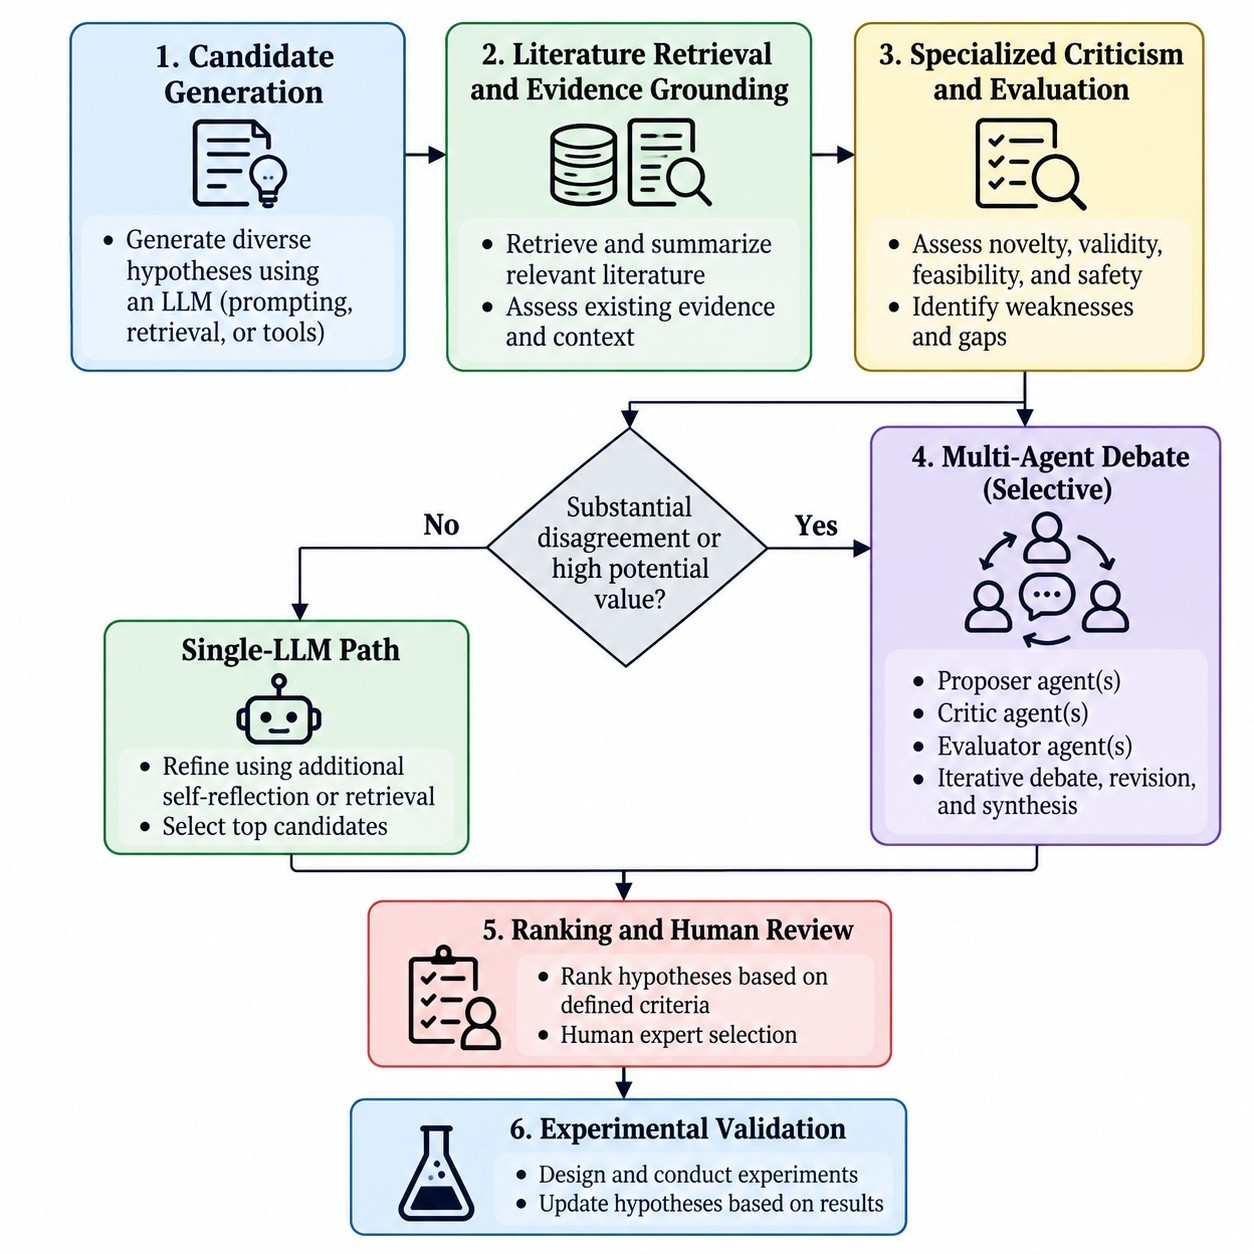
\includegraphics[width=0.9\textwidth]{figures/hybrid-workflow.jpg}
  \caption{A proposed hybrid method of scientific hypothesis generation. It starts by generating candidates with one LLM, then, retrieves literature and evaluates it in a specialized way. Multi-agent debate is turned on when there is significant disagreement among evaluators and/or high potential value in further exploration. Final candidates are ranked and checked against by human experts prior to experimental validation.}
  \label{fig:hybrid-workflow}
\end{figure*}

Future systems should not aim for consensus, but rather, disagreement. They should keep a linkage of claims to papers, observations, assumptions, and proposed tests. They should also give adaptive compute, in which easy cases can be processed by one agent, and more agents, verification would be provided for difficult and high impact cases.

Assessment should be directed towards future standards. A system should be able to formulate some hypotheses before the literature or experimental results are available to it and then it should be judged based on its prediction accuracy. This would set apart true discovery from re-packaging done in hindsight. Lastly, science agents should be constrained with risks, uncertainty that is transparent and human approval before consequential experiments.


\section{Conclusion}
\label{sec:conclusion}

Single LLM and multi-agent debate systems are two very different approaches to scientific hypothesis generation. The single LLM approach is efficient, is very reproducible and can be quite capable when you add in retrieval, self-reflection and scientific tools. The multi-agent approach allows for explicit parallel exploration, role specialisation and criticism. The benefits of this approach are however conditional and can be negated by cost, correlated errors, sycophancy and premature consensus.

The literature therefore points to a conditional rather than a universal conclusion. Multi-agent debate is most valuable when it provides meaningful independence, improves evidence checking or resolves genuine substantive disagreement. Single LLMS may be the better option in the case of rapid exploration, constrained workflows and in situations where the additional interaction doesn't lead to any improvement in validation. In either case the key test is whether the output is novel, evidence based, testable and capable of generating useful scientific knowledge.

\nocite{*}
\bibliographystyle{ACM-Reference-Format}
\bibliography{references}

\end{document}